% Note: remove `openany` for printed version
\documentclass[12pt,a4paper,openany,dutch,english]{extbook}
\usepackage[a4paper,includeheadfoot,margin=2.50cm]{geometry}


% By default, LaTeX tries to stretch whitespace between paragraphs on a page in order to reduce whitespace at the end of the page. This sometimes gives ugly results. The following command disables that stretching.
\raggedbottom % Don't reduce whitespace at the end of a page.

\renewcommand{\baselinestretch}{1.2}  % stretch horizontal space between everything by 20%


\usepackage[hyphens]{url} % Break line on hyphens in long urls
\usepackage{graphicx}
\graphicspath{{images/}}
\usepackage{pdfpages}
\usepackage{enumitem}
\usepackage{float}
\usepackage{caption}
\usepackage{subcaption}
\usepackage[toc,page]{appendix}
\usepackage{fontspec}
\usepackage[T1]{fontenc}

% Don't indent table of contents, list of figures, and list of tables
\usepackage{tocloft}
\setlength{\cftsecindent}{0pt}    % Remove indent for \section in Table of Contents
\setlength{\cftsubsecindent}{0pt} % Remove indent for \subsection in Table of Contents
\setlength{\cftfigindent}{0pt}    % remove indentation from figures in List of Figures
\setlength{\cfttabindent}{0pt}    % remove indentation from tables in List of Tables

\usepackage{parskip} % Add space between two paragraphs and don't indent the first line of the paragraph

% To generate fake lorem ipsum text
\usepackage{lipsum}



%
% UGent style guide
%
\setmainfont[
	Path=fonts/,
	BoldFont      =UGentPannoText-SemiBold.ttf,
	ItalicFont    =UGentPannoText-Normal.ttf,
	ItalicFeatures={FakeSlant=0.3},
	BoldItalicFont=UGentPannoText-SemiBold.ttf,
    BoldItalicFeatures={FakeSlant=0.3},
]{UGentPannoText-Normal.ttf}
\urlstyle{same} % Also use the default font for URLs


% If you want left justified text, uncomment the line below.
%\usepackage[document]{ragged2e} % Left justify all text

% Style Chapter titles so they have the chapter number in grey.
\usepackage{color}
\definecolor{chaptergrey}{rgb}{0.5,0.5,0.5}
\usepackage[explicit, pagestyles]{titlesec}
\titleformat{\chapter}[display]{\bfseries}{\color{chaptergrey}\fontfamily{pbk}\fontsize{80pt}{100pt}\selectfont\thechapter}{0pt}{\Huge #1}
\titlespacing*{\chapter}{0pt}{-80pt}{30pt}


% Header showing chapter number and title and footer showing page number
\newpagestyle{fancy}{%
  \sethead{} % left
          {} % center
          {\Large\thechapter~~\chaptertitle} %right
  \setfoot{} % left
          {\thepage} % center
          {} %right
  \setheadrule{0pt}
}
\pagestyle{fancy}

% Header showing chapter title and footer showing page number
\newpagestyle{numberless}{%
  \sethead{} % left
          {} % center
          {\Large\chaptertitle} %right
  \setfoot{} % left
          {\thepage} % center
          {} %right
  \setheadrule{0pt}
}

% We use the package `minted` for modern code highlighting.
\usepackage[newfloat,chapter]{minted}
\SetupFloatingEnvironment{listing}{name=Codefragment, listname=List of Acronyms}
%\SetupFloatingEnvironment{listing}{name=Code Fragment, listname=List of Code Fragments} % lang:english


\PassOptionsToPackage{hyphens}{url}
\usepackage{hyperref}
\usepackage{url}

\usepackage[numbers]{natbib}       % For bibliography; use numeric citations
\bibliographystyle{IEEEtran}
\usepackage[nottoc]{tocbibind}     % Put Bibliography in ToC

%
% Defines \checkmark to draw a checkmark
%
\usepackage{tikz}
\def\checkmark{\tikz\fill[scale=0.4](0,.35) -- (.25,0) -- (1,.7) -- (.25,.15) -- cycle;}

%
% For tables
%
\usepackage{booktabs}
\usepackage{array}
\usepackage{ragged2e}  % for '\RaggedRight' macro (allows hyphenation)
\newcolumntype{L}[1]{>{\raggedright\let\newline\\\arraybackslash\hspace{0pt}}m{#1}}
\newcolumntype{C}[1]{>{\centering\let\newline\\\arraybackslash\hspace{0pt}}m{#1}}
\newcolumntype{R}[1]{>{\raggedleft\let\newline\\\arraybackslash\hspace{0pt}}m{#1}}

% Fix error "Package hyperref Warning: The anchor of a bookmark and its parent's must not be the same. Added a new anchor on ..."
\newcommand{\sectionbreak}{\phantomsection}

\renewcommand\appendixtocname{Bijlagen}                     % lang:dutch
\renewcommand\appendixpagename{Bijlagen}                    % lang:dutch


\usepackage[toc,acronym]{glossaries}  % for list of acronyms
% \makeglossaries                       % start internal list of acronyms
\makenoidxglossaries
%
% Set the title and your name
%
%%%%%%%%%%%%%%%%%%%%%%%%%%%%%%%%%%%%%%%%%%%%%%%%%%%%%%%%%%%%%%%%%%%%%%
%
% Add the specific info for your thesis
%
%%%%%%%%%%%%%%%%%%%%%%%%%%%%%%%%%%%%%%%%%%%%%%%%%%%%%%%%%%%%%%%%%%%%%%

\title{Standardizing USB in the WebAssembly System Interface}
\author{Wouter Hennen}

%%%%%%%%%%%%%%%%%%%%%%%%%%%%%%%%%%%%%%%%%%%%%%%%%%%%%
% Add all the acronyms you use in your thesis here. %
% These will be added to the List of Acronyms       %
%%%%%%%%%%%%%%%%%%%%%%%%%%%%%%%%%%%%%%%%%%%%%%%%%%%%%

\newacronym{K8S}{K8S}{Kubernetes}
\newacronym{Wasm}{Wasm}{WebAssembly}
\newacronym{WASI}{WASI}{WebAssembly System Interface}
\newacronym{API}{API}{Application Programming Interface}
\newacronym{CPU}{CPU}{Central Processing Unit}
\newacronym{IoT}{IoT}{Internet of Things}
\newacronym{USB}{USB}{Universal Serial Bus}
\newacronym{WIT}{WIT}{Wasm Interface Type}



%
%  END OF HEADER
%  The actual latex document content starts here.
%
\begin{document}
\frontmatter
\pagestyle{empty}

% Download the cover sheet from Plato
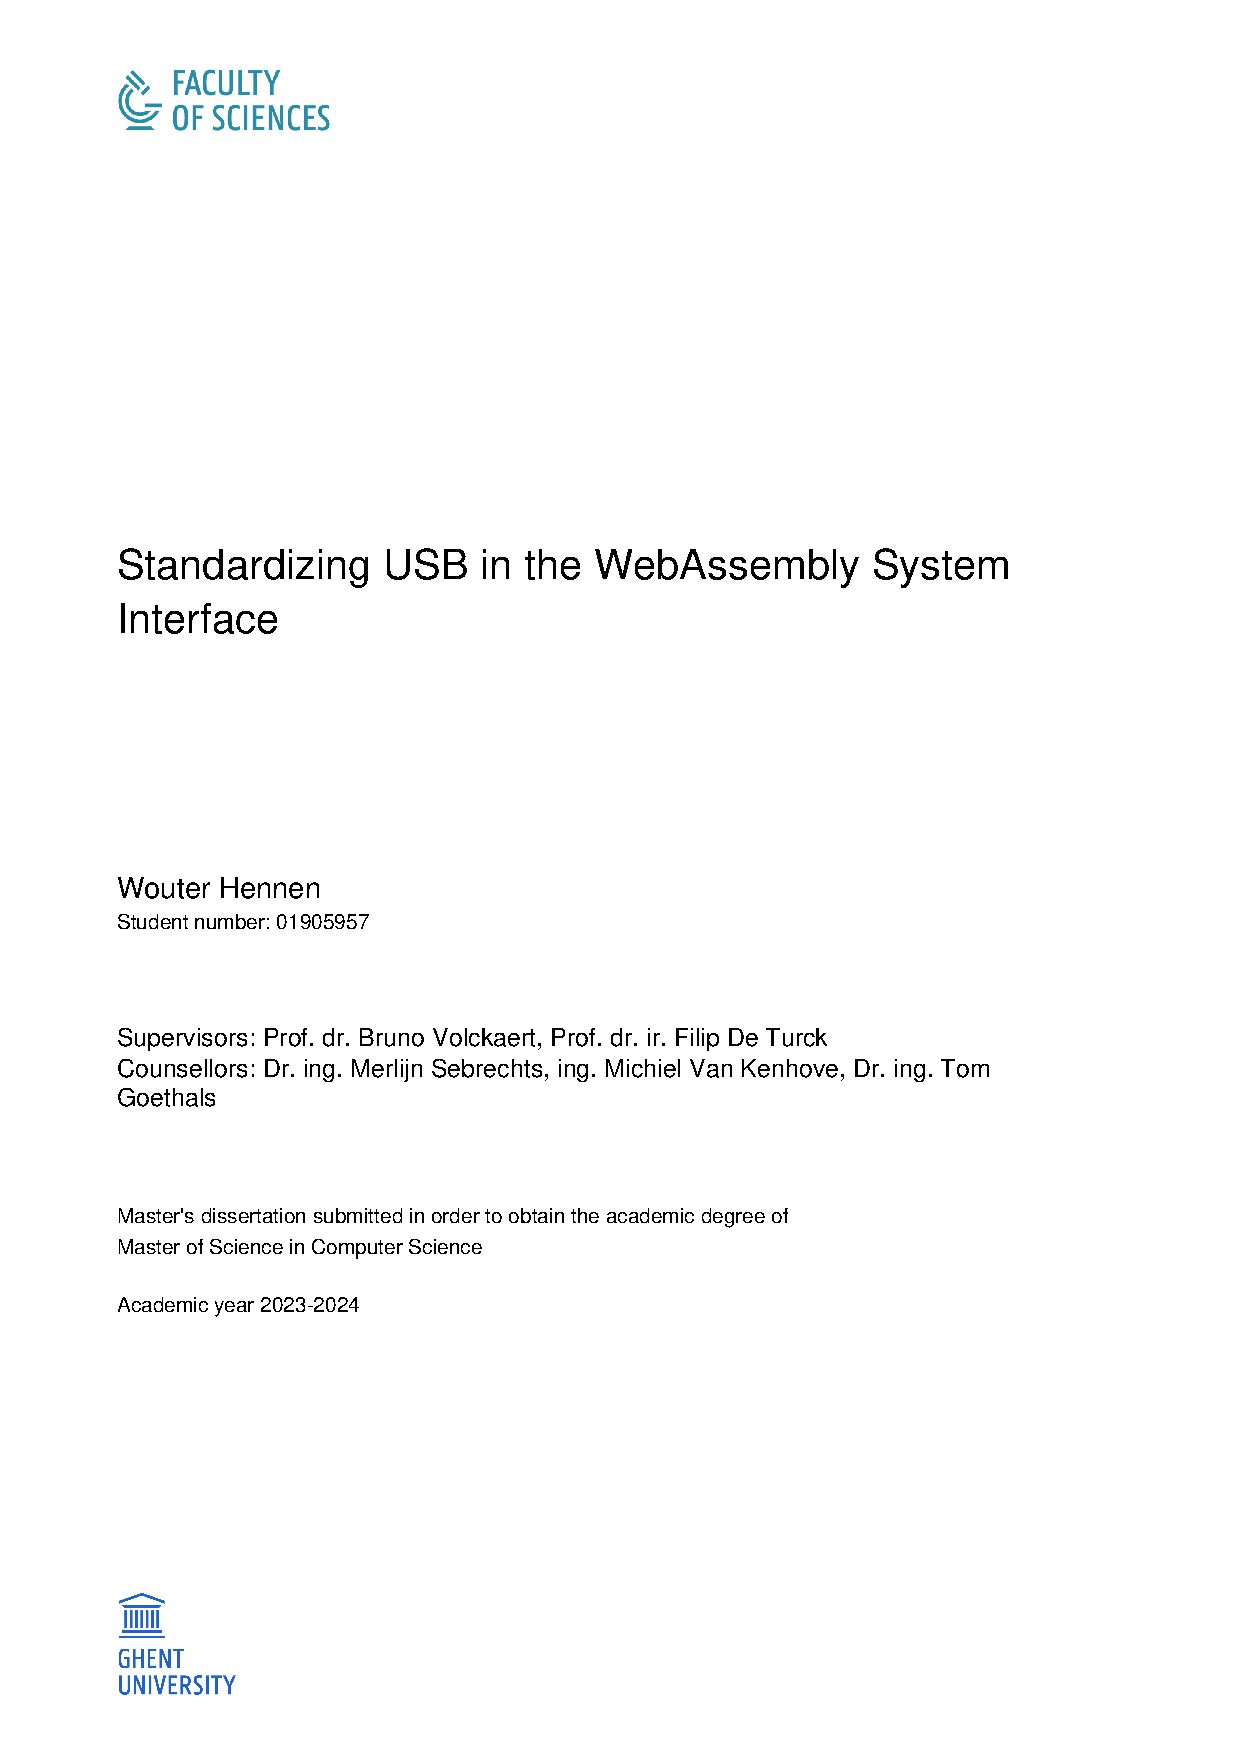
\includepdf{cover-sheet.pdf}

\chapter*{Acknowledgements}
I would like to thank my counsellors Dr. ing. Merlijn Sebrechts and ing. Michiel Van Kenhove for their help, commitment, feedback and time to make this thesis possible.

I would also like to thank my supervisors, Prof. dr. Bruno Volckaert and Prof. dr. ir. Filip De Turck.

Additionally, I would also like to thank my collegue Warre Dujardin for the collaboration on the proposal.

I would like to thank the WASI community for the creation of WIT, the available tooling and support.
\chapter*{Disclaimer regarding the master's thesis}

This master's thesis is part of an examination. Any comments made by the evaluation committee during the oral presentation of the master's thesis were not incorporated into this text.
\chapter*{Abstract}
\chaptermark{Abstract}
\addcontentsline{toc}{chapter}{Abstract}  

Updating software of \acrfull{IoT} devices is currently difficult. Having a longer lifespan than the average gadget, and oftentimes having special hardware and compilers that requires a lot of maintenance, most \acrshort{IoT} devices lose software support too soon \cite{wasi_iot}.
\acrfull{Wasm}, once made to run compiled code in a lightweight virtual machine in the browser, is trying to tackle this problem by expanding its support outside the browser. Because of its near-native performance, security, compactness and language interoperability, \acrshort{Wasm} is gaining popularity for its use on edge devices \cite{wasi_iot}. However, \acrshort{Wasm} lacks a proper interface to use outside the browser. To tackle this issue the \acrfull{WASI} was introduced, with the goal to provide a universal \acrshort{API} for all supported platforms and languages. \acrshort{WASI} is still in development and currently lacks an \acrshort{API} for using USB devices. The goal of this thesis is to research and develop an \acrshort{USB} \acrshort{API} for \acrshort{WASI}.

As part of the development is creating a proposal to extend the standard, where the interface of the \acrshort{API} is laid out and other matter, such as platform support, is further discussed. As part of this thesis, an initial proposal has been created \cite{wasi_usb}. The proposal has advanced to Phase 1 of the proposal process \cite{proposal_phases} and progress is being made to progress to Phase 2. The proposal contains a \acrshort{WIT} interface which supports enumerating devices, reading descriptors, connecting, reading and writing to devices and getting device connection updates. After doing research on existing similar solutions, such as WebUSB \cite{WebUSB} and \cite{LibUSB}, the proposal has taken inspiration from LibUSB. This makes it easier for developers to port existing applications to \acrshort{Wasm} as both LibUSB and \acrshort{WASI} \acrshort{USB} have similar interfaces. Some parts have been made different deliberately, for example the way file handles work. This way, the \acrshort{API} is easier to reason about. As \acrshort{Wasm} is sandboxed by default, access control is provided so programs do not have access to all devices by default. It is up to the user to specify which devices a program can access.

A reference implementation for the \acrshort{API} is provided \cite{wasi_usb} and extends the Wasmtime \cite{wasmtime_website} runtime to provide support for the \acrshort{USB} \acrshort{API}.

The implementation has been evaluated in three ways. First, a functional evaluation was made, testing the functionality of the API. In this evaluation, a guest module will observe connection events for a specific game controller, connect to the game controller, read out its state and control its rumble motors, confirming that the most important parts of the \acrshort{API} work.

Afterwards, the implementation has been evaluated for latency and memory usage. This is done by creating a \acrshort{USB} mass storage device driver by using the \acrshort{WASI} \acrshort{USB} \acrshort{API}. The file tree of a \acrshort{USB} drive can be read out and the file contents can be read. Comparing this against a native implementation shows on average a 4.2\% increase in latency, which is a good result. Memory usage using the \acrshort{WASI} \acrshort{API} is significantly higher, with the program using approx. 70\% more memory during heavy workloads, compared to native. This is likely caused by the way the memory model works in the Component Model, requiring the use of copying of data between components.

The \acrshort{WASI} \acrshort{USB} \acrshort{API} still has a long way to go before it is production ready, but the example programs in this thesis show the possibilities of the \acrshort{API} and demonstrate how the \acrshort{API} can be used in real-world use cases.
% How to add the extended abstract:
%
% You should write the extended abstract as a separate overleaf project. Then compile it there, download the PDF, and upload it to this project.
%
% Use the "IEEE conference proceedings template" to create the extended abstract project. 
% https://www.overleaf.com/latex/templates/ieee-conference-template/grfzhhncsfqn
%
% Then download the final PDF, upload it to the root of this project, and point the statement below to the correct file.
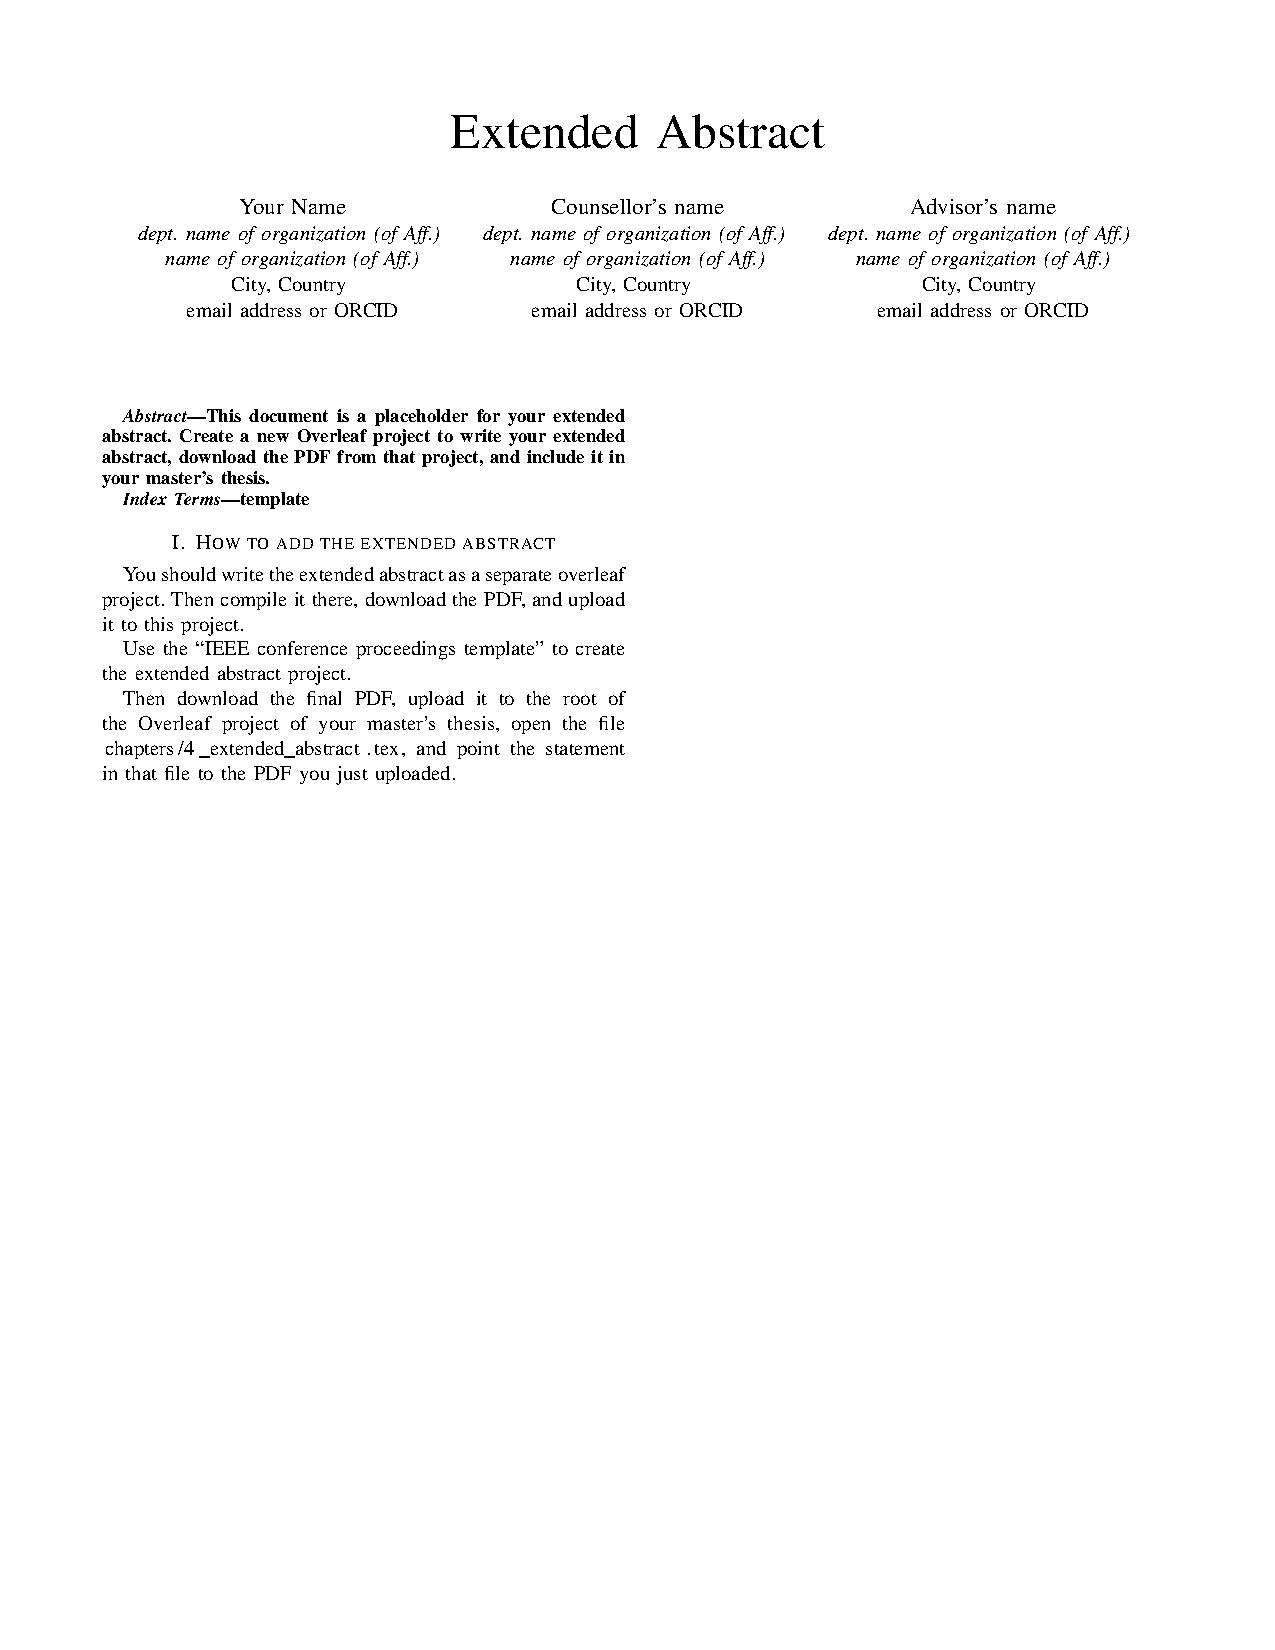
\includepdf[pages={-}]{extended-abstract.pdf}


\tableofcontents\newpage
\listoffigures\newpage
\listoftables\newpage
%%%%%%%%%%%%%%%%%%%%%%%%%%%%%%%%%%%%%%%%%%%%%%%%%%%%%%%%%%%%%%%
%                                                             %
% Note: To add or remove acronyms, modify `personal_data.tex` %
%                                                             %
%%%%%%%%%%%%%%%%%%%%%%%%%%%%%%%%%%%%%%%%%%%%%%%%%%%%%%%%%%%%%%%

\printnoidxglossary[type=\acronymtype, title={List of Acronyms}]
% \printglossary[type=\acronymtype, title={List of Acronyms}] % English

\glsaddallunused[\acronymtype]                              % make sure all unused acronyms are in list

\setlist[description]{style=standard} % reset list settings back to default

\listoflistings\newpage

%
% Include the main chapters of the thesis below
% Note: it's best to avoid spaces in filenames as Latex might complain about them.
%
\mainmatter
\pagestyle{fancy} % Use header
\chapter{Introduction}
\label{chap:intro}

% In today's world, hyperscale cloud providers, such as Microsoft Azure and Amazon Web Services, are used extensively. These companies provide serverless functions, which run for short bursts and close immediately afterwards. In order to do this efficiently, the sandbox in which the code is executed should be able to quickly spin up, so the cold start problem can be minimized. Existing services like Docker and K8S are mostly used for this, but are not ideal: while being more performant than full blown operating systems, there cold boot is still problematic. A new standard, the WebAssembly System Interface (WASI), has been created which should greatly mitigate this problem.
% 
% \acrfull{Wasm} originally started as a way for browsers to execute code written in a language other than Javascript. It allows code from any supported programming language to be compiled to machine instructions for a virtual CPU, and for these instructions to be efficiently executed in the browser sandbox. This has proven to be successful and has opened numerous possibilities for web apps that weren't possible before. A great example of this is the new Google Earth website, which uses WebAssembly underneath, which allows for performant rendering of the Earth.
% 
% This model of running code on a lightweight virtual CPU seen interest outside of the browser, mainly for servers, low power devices (IOT), and so on. There, the WebAssembly System Interface could replace Docker, and provide performance improvements, power and storage savings.
% 
% WASI is currently still in development, and has a long way to go to get stable. One of the problems WASI is currently facing is the lack of APIs available to interface with the system. One of the APIs that is currently missing is the one to interact with USB devices. Having such an API would be useful for servers, cars, IOT devices, etc. The goal of this master's thesis is to create an USB proposal for expanding the WASI, and eventually add support for USB to WASI. With access control, users can decide which devices a program running in WASM can access.


% V2 TEKST

Updating software of \acrfull{IoT} devices is currently difficult. As the devices are home appliances, they are often used for longer periods of time, compared to other tech such as smartphones. As a consequence, these devices need longer software support. In reality, a lot of devices stop getting updates after a few years, making them vulnerable to cyberattacks. When an \acrshort{IoT} device gets hacked, it can be used as part of a botnet, or worse, send sensitive info (such as a video feed) to the attacker. There are multiple causes to why this software support period is short: no standardized updating mechanisms, special hardware and compilers, etc. \cite{wasi_iot}

In Web browsers, \acrfull{Wasm} acts as a generalized layer between the native browser API and a programming language. This model can also be applied outside the browser context and can solve some of the problems of native code. However, in order to do so, some changes are needed. As \acrshort{Wasm} is primarily targeted towards browser applications, it only provides libraries to do those things, for example accessing the DOM. No low-level libraries exist for controlling hardware devices, which would be required for \acrshort{IoT} devices. To solve this, a new specification was created: the \acrfull{WASI}

\acrshort{WASI} is a group of API specifications that can be used with software compiled to \acrshort{Wasm}. These APIs provide a standardized interface for any programming language that can compile to \acrshort{Wasm}. Because the APIs act as a layer between the native APIs and the application, access control can be applied to control what an application can access. To provide APIs that feel natural in any language, a new interface description language was born: \acrfull{WIT}. For each programming language, bindings can be created that expose a generalized API.

With \acrshort{WASI}, standardized APIs can be created that can be used to talk and control hardware. As the APIs are not device specific anymore and no compiling to specific architectures is needed anymore, updating software for \acrshort{IoT} devices has become a lot easier.

\section*{Problem Statement}

The \acrshort{WASI} standard is still in development and currently lacks an API to interact with USB devices. Having an API for USB devices is crucial for \acrshort{IoT} devices as a lot of hardware, such as cameras, will oftentimes communicate over USB.

\section*{Goal}

The goal of this master's thesis is to research and propose a new USB API for \acrshort{WASI}. Special attention will be given to access control, portability and performance.

\section*{Research Questions}

\begin{itemize}

\item What aspects of the USB interface can benefit of access control?

\item In what way can a WASI API be created that makes porting code easy?

\item What is the performance impact of this API compared to native code?

\end{itemize}

\chapter{Background}
\label{chap:rel_work}
In the early days of computers, various connectors existed for computers to communicate with external devices. A few examples of such connectors are the PS/2 port (Primarily used for Mouse / Keyboard) or the Parallel port (Often used for printers). These connectors have varying sizes, shapes and limitations and cannot be used for all devices. Therefore, computers needed to have all these ports, requiring lots of space. To address these issues, the USB connector was introduced. YEars later, the interface has become the de-facto standard for wired device communication. Over the years, USB has evolved with multiple revisions. These revisions focus on key aspects of the interface, such as transfer speeds, power delivery and added functionality. The USB connector has also undergone revisions, making it smaller and reversible, so it is usable on a larger variety of devices.

In this thesis, the focus is on the software side of the USB standard. Therefore, the hardware will not be considered further.

\section{Transferring Data}
\subsection{Pipes}
Data is transferred through pipes. A pipe is a connection from the host controller to the endpoint. Not all pipes are the same: they differ in the bandwidth they support, which transfer types are supported, in which direction data can flow, and their packet and buffer size. Pipes can generally be split up into two kinds.

\subsubsection{Streaming Pipes}
A Streaming Pipe is a one-way communication channel for the host or guest device to send any kind of data to the other end. This pipe is controlled by either the host of or guest device, and data is sent in a sequential way. The isochronous, interrupt and bulk transfer types will use this pipe to send data.

\subsubsection{Message Pipes}
A Message Pipe is a bidirectional communication channel. This pipe allows both the host and guest device to send commands in either direction on the same pipe. All message pipes are controlled by the host device. Only one transfer type supports this pipe: the control transfer type.

\subsection{Transfer Types}
The USB standard defines four transfer types. Each transfer type serves a different purpose, being optimized for speed, latency, correctness or reliability.

\subsubsection{Interrupt Transfer}
Interrupt transfers are most used for devices that transfer small amounts of data frequently. They have a bounded latency and are therefore suited for devices that require low latency and low bandwidth. Interrupt transfers can be initiated by both the host and guest device. The sent data will be queued by the sender, until the receiver polls the device.

Examples of devices that often use interrupt transfers are mice and keyboards.

\subsubsection{Isochronous Transfer}
Isochronous transfers are used for real-time data streaming. They provide a guaranteed data rate, but do not guarantee a correct transfer of data, and data can be lost. This makes the transfer type not suitable for situations where data integrity is important.

Examples of use cases where isochronous data transfer is often used is for audio devices or video streaming.

\subsubsection{Bulk Transfer}
Bulk transfers are suited for transferring large amounts of data where timing is not an issue, but data integrity is. No guarantee on timing is made, but guaranteed correct delivery is.

Examples of use cases for bulk transfers are sending files to printers or storage devices.

\subsubsection{Control Transfer}
Control transfers are used for configuration, command and status operations between the host and guest device. Control transfers operate on the Message pipe and has setup, data and handshake stages. The handshakes guarantee correct delivery, but will lead to a slower transfer speed. Therefore, control transfers are not used to transfer a lot of data, but rather for device initialization and control.

The Control transfer type can be seen as a TCP connection but for USB devices.

\subsection{Descriptors}
\chapter{Titel derde hoofdstuk}
\label{chap:evaluation}

In dit hoofdstuk ...

\section{Sectie titel}
\label{sec:scalable_faafo}

Vul aan...

\chapter{Titel vierde hoofdstuk}

In dit hoofdstuk ...

\section{Sectie titel}

Vul aan ...

\section{Sectie titel2}

Vul aan ...

\subsection{Subtitel}
Vul aan ...
\chapter*{Conclusie}
\chaptermark{Conclusie}
\addcontentsline{toc}{chapter}{Conclusie}  

Vul aan...

\phantomsection
\section*{Ethische en maatschappelijke reflectie}
\addcontentsline{toc}{section}{Ethische en maatschappelijke reflectie}  

Deze sectie is enkel vereist voor de opleidingen industrieel ingenieur. De locatie van deze sectie lichtjes af van de volgorde voorgeschreven door de faculteit. Wij raden aan om deze reflectie als deel van de conclusie te maken omdat je daardoor eenvoudig kan refereren naar resultaten in je masterproef zelf.

Meer informatie kan je opzoeken op https://www.sdgs.be/nl/sdgs




\renewcommand\bibname{Referenties}
\bibliography{referenties}


\pagestyle{numberless} 
\pagestyle{empty}
\begin{appendices}
\section*{Bijlage A}
\addcontentsline{toc}{section}{Bijlage A}  

Toelichting bijlage.



\newpage
\section*{Bijlage B}
\addcontentsline{toc}{section}{Bijlage B}  

Toelichting bijlage.

\end{appendices}


\end{document}
